\chapter{Objectives}
\label{chap:2_objectives}
Once we have presented the introductory context of this project, we will describe its objectives, along to the followed methodology to achieve all of them.\\

The final objective is to enrich the JdeRobot platform on its Computer Vision aspect, upgrading an existing tool and creating two consecutive new ones. All of them will be focused on \emph{applying deep learning on a real time operation}. Keeping this in mind, we will be able to generate a behavioral focused, as a final application, on tracking and actively following a person, making use of a robot. This internal process of transformation of a stimulus into a reactive movement will be accomplished using \textit{Convolutional Neural Networks}.\\


\section{Milestones to achieve}
	 \begin{enumerate}
	 	\item \emph{Classification tool, for processing live images.}
			Our first objective (and the first task to tackle) will be to upgrade the support of the digit classification tool already existent in JdeRobot, \texttt{DigitClassifier} (\autoref{sec:3_digitclassifier_jderobot}). This will allow us to augment the scope of this component, due to the support for the new framework, TensorFlow (\autoref{sec:3_tensorflow}). This is a good starting point to achieve some initial skills building and training Convolutional Neural Networks on TensorFlow (it will be the main framework used all along the project).\\
		
		\item \emph{Detection tool, for processing live images.}
			As it will be described on the suitable chapter, we will build a new tool (\texttt{ObjectDetector}) which deploys \textit{a generic object detection algorithm} on an incoming video stream. This component will be ready to work in \emph{real time}. It will also be compatible with new network models (e.g. a chosen one suitable for the purpose), which will be loaded transparently at runtime.\\
			
			As it can be inferred, the tool will not provide a response \textit{per se}. Its visible output will be to draw \emph{bounding boxes} surrounding each detected object, indicating as well the class where that particular object belongs (person, airplane, dog, etc.), and its score (confidence in \%).\\
			
			
		\item \emph{Application of neural detection inside a robotic behavioral}
		
			As an example of the plethora of possible applications of the previous described objective/milestone (object detection on an image), we want to implement a ``person following" behavioral. Our main objective here is to \textit{identify and track} the person to follow, which will semantically be called \emph{mom}. This component, \texttt{FollowPerson}, will rely for this on the previous tool, \texttt{ObjectDetector}. The great advantage here is the strength a CNN can achieve under variable light conditions. That makes this technique perfectly suitable to command physical actuators on a robot.\\
			
			We will make use of the detected people (with the technique followed on the previously described node and constraining the result to only retain people detection), and look for the face of each one of them, in order to distinguish which one is \emph{mom}, in case it is being seen by the camera, and command a proper response to the robot with the objective of following \emph{mom}.\\
		\end{enumerate}

As we have said before, these two last milestones are successive. Thus, they will share an important part of the global objectives.\\


\section{Methodology}
The development of this project, as it has been described, has been subdivided into smaller tasks, or \emph{prototypes}, which could be addressed as individual tasks to achieve. The way to tackle them has been a \textit{spiral methodology} \cite{boehm-spiral}.\\

\begin{figure}[h]
	\centering
	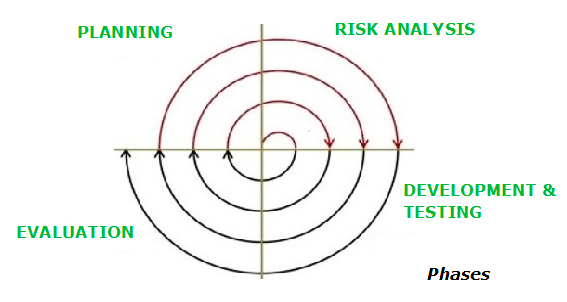
\includegraphics[width=4in]{images/spiral}
	\caption{Spiral Development Model.}
	\label{fig:2_spiral}
\end{figure}

This consists on a software development work procedure that, on a general outline, is very similar to a conch. It describes a 4 phases methodology \cite{spiral-steps}, explained right below:

\begin{enumerate}
	\item \textit{Planning:} establishing the objectives to tackle on the incoming work iteration.

	\item \textit{Risk Analysis:} Later, we evaluate the possible risks and dangers we can find developing the specific program(s). For each found risk, we will try to find a solution to solve or, at least, mitigate it beforehand.

	\item \textit{Development \& testing\footnote{\textit{"In theory, theory and practice are the same. In practice, they are not."}, Y. Berra}:} This phase is purely focused on writing the planned piece of software, following the guidelines obtained on the previous steps. In addition, corresponding tests should be performed to check that the work will accomplish the asked functionality.
	\item \textit{Evaluation:} Lastly, when the development phase has been finished, an evaluation has to be performed on the results. This will be the key to know if it is compliant with the initial requirements and if, hence, its development has been successful.
\end{enumerate}

As this was the general procedure followed for each iteration of the developed software, the completion of the evaluation phase immediately led to another planning phase, already belonging to the next iteration. As this is a cyclic process, we can perform as many iterations as desired, slightly increasing the scope of the project on each new one.\\

The workflow present on this project has been supported by weekly meetings, scheduled in order to get up-to-date with the last established objectives and tasks, and set up the work until the next one. This has allowed to keep a constant feedback with the tutor and hold the followed path onto the desired direction.\\


Additionally, a MediaWiki page\footnote{\url{https://jderobot.org/Naxvm-tfg}} has been mantained on the JdeRobot website, reflecting every effort and achievement in order to have a good temporal reference of the work done, and a timeline of accomplishments, and including demonstration videos for each successful iteration result.\\

The code for all the project has been handled on the GitHub repository\footnote{\url{https://github.com/RoboticsURJC-Students/2017-tfg-nacho\_condes}} created for this purpose. However, as the resulting nodes were officially incorporated to the JdeRobot environment, they were migrated to their own repositories. This will be further described on the section dedicated to each component/iteration.\\


\section{Requirements}
\label{sec:2_requirements}
For every covered topic, the developed solution must be compliant with the requirements formulated below:

\begin{itemize}
	\item As each tool/application will need to perform simultaneous tasks (which, in addition, require a very unbalanced computation load), it will be implemented with several asynchronous \emph{threads}, with different tunable update periods. The asynchronism will \emph{prohibite blocking calls between them}, as that would stop independent threads (e.g. it's senseless that the \emph{GUI} had to wait the \emph{CNN} to finish before updating the window). So, this will be kept in mind for data exchange as well.\\
	
	In particular, the thread controlling the neural networks will have the capability to \emph{be stopped and resumed on demand}, having the user several buttons for this (stop/continue, or perform a single inference on the current image).\\
	
	\item The implemented solutions will be easy to execute for other purposes. This leads to pursue the easiest installation and configuration methods possible.\\
	
	The installation of the required framework can be performed automatically executing the \texttt{pip} Python package manager. The project repository includes a file to install all the dependencies automatically with \texttt{pip install -r requirements.txt}.\\
	
	With respect to the configuration, it has been implemented on a YML format (which will be explained later), allowing a configuration on a human-readable format.
	
	\item The camera implemented in the robot will be on a low height, looking slightly upwards in order to detect faces correctly. So, sometimes it will be such a harsh situation for the detection systems due to lighting issues, encountering situations as tough as on \autoref{fig:2_light_ko}.
	
	\begin{figure}[h]
		\centering
		\begin{subfigure}[b]{0.4\linewidth}
			\centering
			
\includegraphics[width=2.7in]{images/light_ko}
		\end{subfigure}
		\hfill
		\begin{subfigure}[b]{0.5\linewidth}
			\centering
			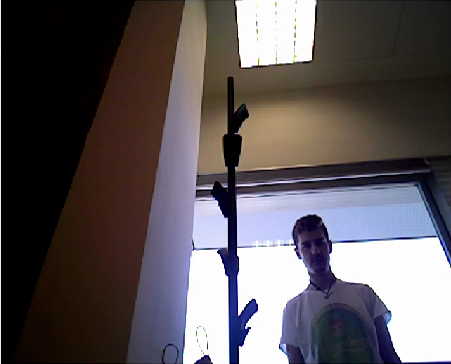
\includegraphics[width=3.3in]{images/light_ko_2}
		\end{subfigure}		
		
		\caption{Hard situations for facial detection, due to light.}
		\label{fig:2_light_ko}
	\end{figure}
	
	The implemented solutions will have to be able to struggle with these situations, which can be feasible due to the position issue, offering a robust response even when there is a strong source of light burning the image.
	
	\item Created neural networks will have to be \emph{generic} (capable of loading a previously saved or imported model), and \emph{persistent}, which means, able to process more than a single frame (unlike many detection solutions findable through a simple Google search).
	
	\item All the proposed solutions, and its subsystems must be capable of running on the available processing hardware:
	\begin{itemize}
		\item \emph{CPU:} Intel i5 4210-U
		\item \emph{RAM:} 8 GB DDR3L
		\item \emph{GPU:} discrete Nvidia 940M (CUDA capabilities: 5.0)
	\end{itemize}
	
	\item Every implemented system must maintain the compatibility with Keras framework: another generic and transparent loader must be written. This selection (TensorFlow/Keras) will be chosen inside the previously mentioned YML configuration file.
\end{itemize}
